\documentclass[a4paper,12pt]{report}

\usepackage[lmargin=2.00000cm,rmargin=2.0000cm,tmargin=5.5000cm,bmargin=2.500000cm,headheight=3.5cm]{geometry}        %Flexible and complete interface to document dimensions
\usepackage[utf8]{inputenc}
\usepackage[T1]{fontenc}
%\usepackage[latin1]{inputenc}
\usepackage{amsmath}
\usepackage{amsfonts}
\usepackage{amssymb}
\usepackage{lmodern}
\usepackage{float}
\usepackage{graphicx}

\usepackage[english,french]{babel}        %use for the below package `datetime'
\usepackage[babel=true]{csquotes}
\usepackage{datetime}        %Change format of `\today' with commands for current time
\renewcommand{\dateseparator}{-}
\newcommand{\headertoday}{\twodigit\day \dateseparator \twodigit\month  \dateseparator \the\year}

\usepackage{animate}
\usepackage{lastpage}
\usepackage{array}
\usepackage{lastpage}
\usepackage{multirow}
\usepackage{titling}
\usepackage{placeins}
\usepackage{media9}
\usepackage{eurosym}
\usepackage{pdflscape}
\usepackage{color}
\usepackage[table]{xcolor}
\definecolor{mon_bleu}{rgb}{0.137,0.466,0.741}
\definecolor{mon_vert}{rgb}{0.07843,0.4627,0.07843}
\definecolor{mon_rouge}{rgb}{0.62745,0.16078,0.27058}		
%\usepackage{subfigure}
\usepackage{subcaption}

\usepackage[ 
           hidelinks,
           colorlinks=true,
           linkcolor=blue,          % color of internal links (change box color with linkbordercolor)
    	   citecolor=blue,        % color of links to bibliography
    	   filecolor=blue,      % color of file links
    	   urlcolor=blue,           % color of external links
           pdfhighlight =/O]{hyperref}																		% dvipdfm package pour lien hypertextes dans pdf (pdfhighlight--> afficher la main dans le pdf, colorlinks--> colorlinks=true afficher les liens en couleurs)
  
\usepackage{blindtext}
\usepackage[final]{pdfpages}
\usepackage[french]{cleveref}																				% à placer après hyperref attention ne pas utiliser ":" dans les labels des équations avec French babel activé et cref

\usepackage{fancyhdr}
%%%%%%%%%%%%%%%%%%%%%%%%%%%%%%%%%%%%%%%%%%%%%%%%%%%%%%%%%%%%%%%%%%%%%%%%%%
%                         FORMAT PERSONNALISES                           %
% %%%%%%%%%%%%%%%%%%%%%%%%%%%%%%%%%%%%%%%%%%%%%%%%%%%%%%%%%%%%%%%%%%%%%%%%

\parindent=0pt        %leading space for paragraphs
\pagestyle{fancy}
\renewcommand{\arraystretch}{1.5}
\renewcommand{\headrulewidth}{0pt}
\fancyhead[CE,CO,LE,LO,RE,RO]{} %% clear out all headers
\fancyhead[C]{%
\begin{tabular}{|m{3.0cm}|m{10cm}|c@{}|}
\hline
\multirow{2}{*}{\includegraphics[scale=0.045]																			% LOGO LABO
{Logo-Symme.png}}& \centering \multirow{2}{*}{ \Large{\thetitle}}  &  \multirow{2}{*}{Page: \thepage ~/ \pageref{LastPage}}\\
& &  \\
\hline
%Etabli par: \newline \theauthor & \multicolumn{2}{l|}{Diffusion: interne}\\
%\hline
\multicolumn{2}{|l|}{Objet: \thetitleobject }& Date: \headertoday ~~\\ 
\hline
\end{tabular}
}
\renewcommand\footrulewidth{1pt}
\fancyfoot[L]{Document confidentiel} 																		% DOCUMENT CONFIDENTIEL
\fancyfoot[R]{Laboratoire SYMME}		 																	% NOM DU LABO

\newcolumntype{x}[1]{>{\centering\hspace{0pt}}p{#1}}
\setlength{\doublerulesep}{\arrayrulewidth} 


\usepackage{tikz}																							% pour les diagrammes
\usetikzlibrary{calc}
\usetikzlibrary{shapes.geometric,shapes.arrows,decorations.pathmorphing}
\usetikzlibrary{matrix,chains,scopes,positioning,shapes,arrows,fit}
\usetikzlibrary{calc,decorations.pathreplacing}
\usetikzlibrary{calc}
\usetikzlibrary{backgrounds,decorations.markings}

\setcounter{secnumdepth}{5}		%sous sous sous section



%%%%%%%%%%%%%%%%%%%%%%%%%%%%%%%%%%%%%%%%%%%%%%%%%%%%%%%%%%%%%%%%%%%%%%%%%%%%%%%%%%%%
%%-------------> PAGE DE GARDE INFO
%%%%%%%%%%%%%%%%%%%%%%%%%%%%%%%%%%%%%%%%%%%%%%%%%%%%%%%%%%%%%%%%%%%%%%%%%%%%%%%%%%%%

\author{Auteur}
\newcommand{\validator}{J. COLLOMB}
\title{Rapport d'avancement}
\selectlanguage{french}	
\date{\today}
\newcommand{\thetitleobject}{Comment intégrer des modèles 3D ?}
\setcounter{tocdepth}{6}
\setcounter{secnumdepth}{6}


%%%%%%%%%%%%%%%%%%%%%%%%%%%%%%%%%%%%%%%%%%%%%%%%%%%%%%%%%%%%%%%%%%%%%%%%%%%%%%%%%%%%
%%-------------> DEBUT DU DOCUMENT 
%%%%%%%%%%%%%%%%%%%%%%%%%%%%%%%%%%%%%%%%%%%%%%%%%%%%%%%%%%%%%%%%%%%%%%%%%%%%%%%%%%%%

\begin{document}

\graphicspath{{Figures/}}

%%%%%%%%%%%%%%%%%%%%%%%%%%%%%%%%%%%%%%%%%%%%%%%%%%%%%%%%%%%%%%%%%%%%%%%%%%%%%%%%%%%%
%%-------------> PAGE DE GARDE 
%%%%%%%%%%%%%%%%%%%%%%%%%%%%%%%%%%%%%%%%%%%%%%%%%%%%%%%%%%%%%%%%%%%%%%%%%%%%%%%%%%%%
\begin{titlepage}
    \centering
    \vspace*{3cm}
    {\bfseries\Large
        \thetitle\\
        \thetitleobject\\
        --- \\
        Document confidentiel\\  																			% LIGNE "CONFIDENTIEL"
        \vskip2cm
    }
    
\includegraphics[scale=0.65]{logos.png}  																% LOGOS DES PARTENAIRES
    \vfill
    \begin{center}
    \begin{table}[b]
    \begin{tabular}{x{.225\linewidth}|| x{.225\linewidth}|| x{.225\linewidth} || x{.225\linewidth} }
    \hline \hline
    \textbf{Date} & \textbf{Révision} & \textbf{Rédigé par} & \textbf{Validé par} \tabularnewline
    \hline \hline
    \thedate & Rev. A  &  \theauthor &  \validator \tabularnewline
    \hline
    ~ & ~ & ~ & ~ \tabularnewline
    \hline
    ~ & ~ & ~ & ~ \tabularnewline
    \hline
    ~ & ~ & ~ & ~\tabularnewline         
    \hline \hline                                                                   
    \end{tabular}
    \end{table}
    \end{center}
    \vfill
    \vfill
    \begin{tikzpicture}[remember picture,overlay]
    \node (label) at (8cm,20cm){
        
\includegraphics[width=2.5cm]{Logo-Symme.png} 													% LOGO LABO
      };
    
	\draw[very thick]
		([yshift=-25pt,xshift=25pt]current page.north west)--
		([yshift=-25pt,xshift=-25pt]current page.north east)--
		([yshift=25pt,xshift=-25pt]current page.south east)--
		([yshift=25pt,xshift=25pt]current page.south west)--cycle;
    \end{tikzpicture}
\end{titlepage}


%\begin{titlepage}
%    \centering
%    
%    \vspace*{3cm}
%    {\bfseries\Large
%        \thetitle\\
%        \thetitleobject\\
%        \vskip2cm
%    }    
%    \vfill
%    \begin{center}
%    \begin{table}[b]
%    \begin{tabular}{x{.225\linewidth}|| x{.225\linewidth}|| x{.225\linewidth} || x{.225\linewidth} }
%    \hline \hline
%    \textbf{Date} & \textbf{R�vision} & \textbf{R�dig� par} & \textbf{Valid� par} \tabularnewline
%    \hline \hline
%    \thedate & Rev. A  &  \theauthor &  \validator \tabularnewline
%    \hline
%    ~ & ~ & ~ & ~ \tabularnewline
%    \hline
%    ~ & ~ & ~ & ~ \tabularnewline
%    \hline
%    ~ & ~ & ~ & ~\tabularnewline         
%    \hline \hline                                                                   
%    \end{tabular}
%    \end{table}
%    \end{center}
%    \vfill
%    \vfill
%    \begin{tikzpicture}[overlay,remember picture]
%    \node (label) at (6.7cm,19.5cm){
%        \includegraphics[width=4cm]{../Figures/logo_CT1.pdf} % also works with logo.pdf
%      };
%    
%    \draw [line width=1pt,rounded corners=7pt]
%        ($ (current page.north west) + (1.5cm,-1.5cm) $)
%        rectangle
%        ($ (current page.south east) + (-1.5cm,1.5cm) $);
%        
%%	\draw[very thick]
%%		([yshift=-25pt,xshift=25pt]current page.north west)--
%%		([yshift=-25pt,xshift=-25pt]current page.north east)--
%%		([yshift=25pt,xshift=-25pt]current page.south east)--
%%		([yshift=25pt,xshift=25pt]current page.south west)--cycle;
%    \end{tikzpicture}
%\end{titlepage}


%%%%%%%%%%%%%%%%%%%%%%%%%%%%%%%%%%%%%%%%%%%%%%%%%%%%%%%%%%%%%%%%%%%%%%%%%%%%%%%%%%%%
%%-------------> SOMMAIRE
%%%%%%%%%%%%%%%%%%%%%%%%%%%%%%%%%%%%%%%%%%%%%%%%%%%%%%%%%%%%%%%%%%%%%%%%%%%%%%%%%%%%

\renewcommand\contentsname{Sommaire}
\setcounter{chapter}{1}
\tableofcontents
%\listoffigures
%\listoftables


%%%%%%%%%%%%%%%%%%%%%%%%%%%%%%%%%%%%%%%%%%%%%%%%%%%%%%%%%%%%%%%%%%%%%%%%%%%%%%%%%%%%
%%-------------> CORPS DOCUMENT
%%%%%%%%%%%%%%%%%%%%%%%%%%%%%%%%%%%%%%%%%%%%%%%%%%%%%%%%%%%%%%%%%%%%%%%%%%%%%%%%%%%%

%-----------------------------------------------------------------------------------
%-----------------------------------------------------------------------------------
\newpage

\section{Générer un modèle 3D}
\subsection{Package et formats requis}
Le package utilisé pour l'intégration d'un modèle 3D est : media9. \\
La commande à placer en début de document est donc : \verb|\usepackage{media9}| \\

Le package media9 permet l'intégration des fichiers \verb|.u3d| et \verb|.prc|. \\
Il est donc nécessaire de générer un modèle 3D à ce format. \\

Des logiciels ne permettent l'export à ce format (ex : SolidWorks), il est donc nécessaire de mettre en place des étapes intermédiaires. Une proposition de démarche est présentée ci-après.

\subsection{Suggestion de démarche}

La démarche proposée repose sur 4 étapes :
\begin{enumerate}
\item Générer le modèle 3D;
\item Exporter dans un format d'échange : \verb|.stl| par exemple;
\item Convertir ce fichier au format \verb|.u3d| à l'aide d'un logiciel externe, \href{http://www.meshlab.net/}{Meshlab} par exemple;
\item Intégrer ce fichier dans \LaTeX.
\end{enumerate}

\subsection{Code \LaTeX}
Un exemple de code est présenté ci-après. Pour plus de détails, voici la \href{http://texdoc.net/texmf-dist/doc/latex/media9/media9.pdf}{documentation} du package avec des exemples. \\

\verb|% Intégration du modèle| \\
\verb|\begin{figure}[hbtp] | \\
\verb|\begin{center} | \\
\verb|\includemedia[ | \\
\verb|label=figure_modele, | \\
\verb|width=0.85\linewidth,height=0.85\linewidth, | \\
\verb|activate=pagevisible, | \\
\verb|3Dpartsattrs=keep, | \\
\verb|3Dnavpane, | \\
\verb|3Dviews={Figures/dynamique/modele.vues} | \\
\verb|]{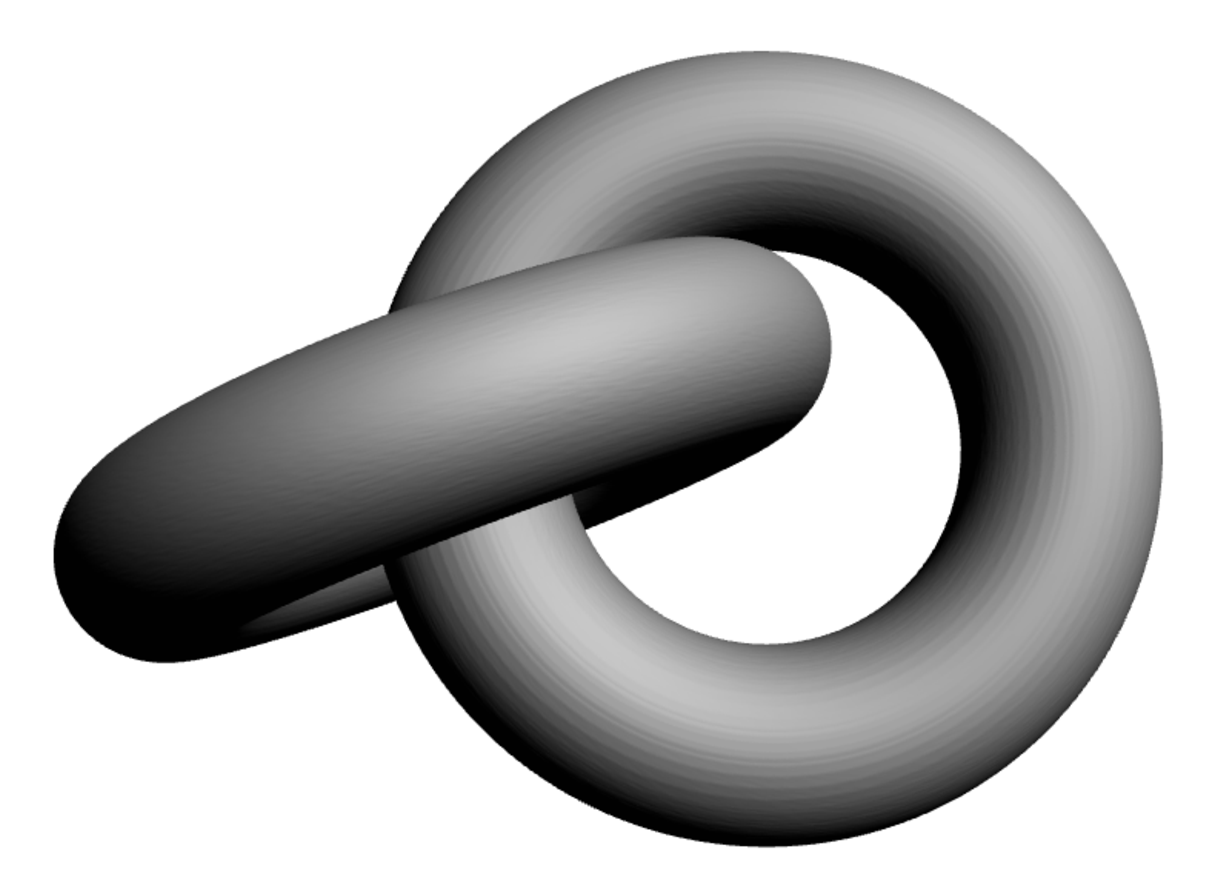
\includegraphics{modele.pdf}}{/dynamique/modele.u3d} | \\

\verb|% Création des boutons cliquables| \\
\verb|\mediabutton[3Dgotoview=figure_modele:0]{\fbox{Vue par défaut}} | \\
\verb|\mediabutton[3Dgotoview=figure_modele:1]{\fbox{Vue de face}} | \\
\verb|\mediabutton[3Dgotoview=figure_modele:2]{\fbox{Vue du maillage}} | \\
\verb|\mediabutton[3Dgotoview=figure_modele:3]{\fbox{Vue en transparence}} | \\

\verb|\end{center}   | \\
\verb|\caption{Exemple de vues dynamiques | \\
\verb|\label{figure_modele_dynamique}}  | \\
\verb|\end{figure} | \\


\section{Exemple}
Un exemple de vue dynamique / interactive est présenté Figure.~\ref{figure_modele_dynamique}. Pour son bon fonctionnement, il est nécessaire d'activer les formulaires et cliquez sur l'image si nécessaire pour charger la visualisation; les zooms et translations sur le modèle sont disponibles.

\begin{figure}[hbtp]
\begin{center}
\includemedia[
label=figure_modele,
width=0.85\linewidth,height=0.85\linewidth,
activate=pagevisible,
3Dpartsattrs=keep,
3Dnavpane,
3Dviews={Figures/dynamique/modele.vues}
]{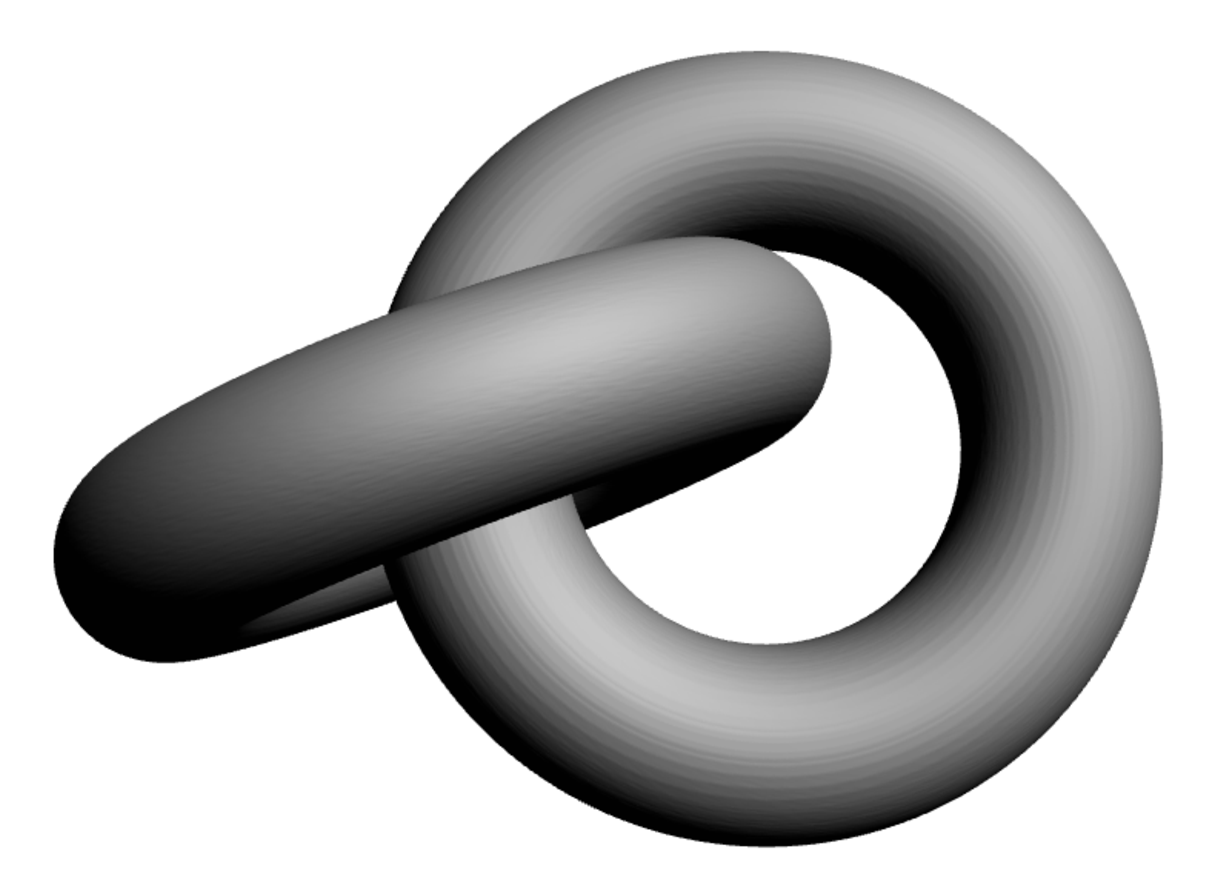
\includegraphics{modele.pdf}}{/dynamique/modele.u3d}

\mediabutton[3Dgotoview=figure_modele:0]{\fbox{Vue par défaut}}
\mediabutton[3Dgotoview=figure_modele:1]{\fbox{Vue de face}}
\mediabutton[3Dgotoview=figure_modele:2]{\fbox{Vue du maillage}}
\mediabutton[3Dgotoview=figure_modele:3]{\fbox{Vue en transparence}}

\end{center}  
\caption{Exemple de vues dynamiques
\label{figure_modele_dynamique}} 
\end{figure}



%%%%%%%%%%%%%%%%%%%%%%%%%%%%%%%%%%%%%%%%%%%%%%%%%%%%%%%%%%%%%%%%%%%%%%%%%%%%%%%%%%%%
%%-------------> FIN DU DOCUMENT
%%%%%%%%%%%%%%%%%%%%%%%%%%%%%%%%%%%%%%%%%%%%%%%%%%%%%%%%%%%%%%%%%%%%%%%%%%%%%%%%%%%%

\end{document}